\documentclass[12pt]{article}

\usepackage[latin1]{inputenc}	% Required for inputting international characters
\usepackage[T1]{fontenc} 		% Output font encoding international characters
\usepackage[english]{babel}
\usepackage{lmodern}
\usepackage{graphicx}  			% to include graphics
\usepackage{authblk} 			% affiliations
\usepackage{authblk}
\usepackage{wrapfig}
\usepackage{enumitem}           % editing lists
\usepackage{amsmath}			% math formulas
\usepackage{hyperref}			% weblinks

\usepackage[
	backend = biber,
	bibencoding = latin1,
	style = authoryear,
]
{biblatex}


\addbibresource{references3.bib}  % add library manually via texmaker

\title{Example}
\author{Me}
\date{\today}


\begin{document} 

\begin{titlepage} % Suppresses headers and footers on the title page

	\centering % Centre everything on the title page
	
	\scshape % Use small caps for all text on the title page
	
	\vspace*{\baselineskip} % White space at the top of the page
	
	%------------------------------------------------
	%	Title
	%------------------------------------------------
	
	\rule{\textwidth}{1.6pt}\vspace*{-\baselineskip}\vspace*{2pt} % Thick horizontal rule
	\rule{\textwidth}{0.4pt} % Thin horizontal rule
	
	\vspace{0.75\baselineskip} % Whitespace above the title
	
	{\LARGE Title name in here} % Title
	
	\vspace{0.75\baselineskip} % Whitespace below the title
	
	\rule{\textwidth}{0.4pt}\vspace*{-\baselineskip}\vspace{3.2pt} % Thin horizontal rule
	\rule{\textwidth}{1.6pt} % Thick horizontal rule
	
	\vspace{2\baselineskip} % Whitespace after the title block
	
	%------------------------------------------------
	%	Subtitle
	%------------------------------------------------
	
	Enter subtitle here
	
	\vspace*{3\baselineskip} % Whitespace under the subtitle
	
	%------------------------------------------------
	%	Editor(s)
	%------------------------------------------------
	
	Edited By
	
	\vspace{0.5\baselineskip} % Whitespace before the editors
	
	{\scshape\Large First Author \\ Second Author \\} % Editor list
	
	\vspace{0.5\baselineskip} % Whitespace below the editor list
	
	\textit{Dragonfly Data Science \\ Wellington} % Editor affiliation
	
	
	%------------------------------------------------
	%	Publisher
	%------------------------------------------------
	
	
	\vspace{0.3\baselineskip} % Whitespace under the publisher logo
	
	2021 % Publication year
	
	{\large publisher} % Publisher

\end{titlepage}




\begin{abstract}
\noindent The aim of this study was to improve our understanding of the role of subalpine microhabitat variability in controlling upper forest limits in abrupt treeline position and identify environmental variables limiting Nothofagaceae regeneration in New Zealand. Results of this study have revealed novel insights into abrupt alpine treelines dynamics where subalpine regeneration is limited by cold-induced photoinhibition and the paucity of favourable microhabitats. The findings elucidate the complex link between biotic and abiotic limitations exposed on different temporal and spatial scales to operate as a sharpening agent in abrupt treeline ecotones.
\end{abstract}

\tableofcontents

\section{Introduction}

\noindent \textit{Fuscospora cliffortioides} regeneration patterns in the subalpine revealed a preference for seedlings to recruit in warmer zones with a reduced risk to experience low minimum temperatures. Exposure to high temperature fluctuations was reduced in subalpine vegetation and revealed species-specific differences. Periodic low-temperature dips are observed throughout the year. Modelling suggested enhanced seedling regeneration above treeline if suitable thermal microclimates limited the expression of macroscale-imposed low temperature dips. A similar directional positive feedback was observed in the projected global warming scenarios.\\
\indent This research shows that for the Nothofagaceae treeline in New Zealand, the current treeline position is constrained by cold-induced photoinhibition effects linked to the surprising occurrence of frequent summer frosts at treeline. As F. cliffortioides is otherwise well-adapted for high altitude environments, suggesting that we will observe a rapid uphill encroachment once current limitations diminish in the face of global warming. Such empirical results, combined with greater use of agent-based modelling that incorporates fine-scale topographic maps and microhabitat heterogeneity will assist us to put individual tree performance in the context of large scale abiotic functional stress gradients and improve our understanding of alpine ecotone formation and maintenance (\cite{barnas_comparison_2019}).Figures and tables can be referenced in LaTeX using the ref command, e.g. Figure \ref{fig:leiden}. 

%%%% FIGURE INSERT %%%%%%%

\begin{figure}[ht]  %t for top, b bottom, h for right here after text
\centering % centers the picture
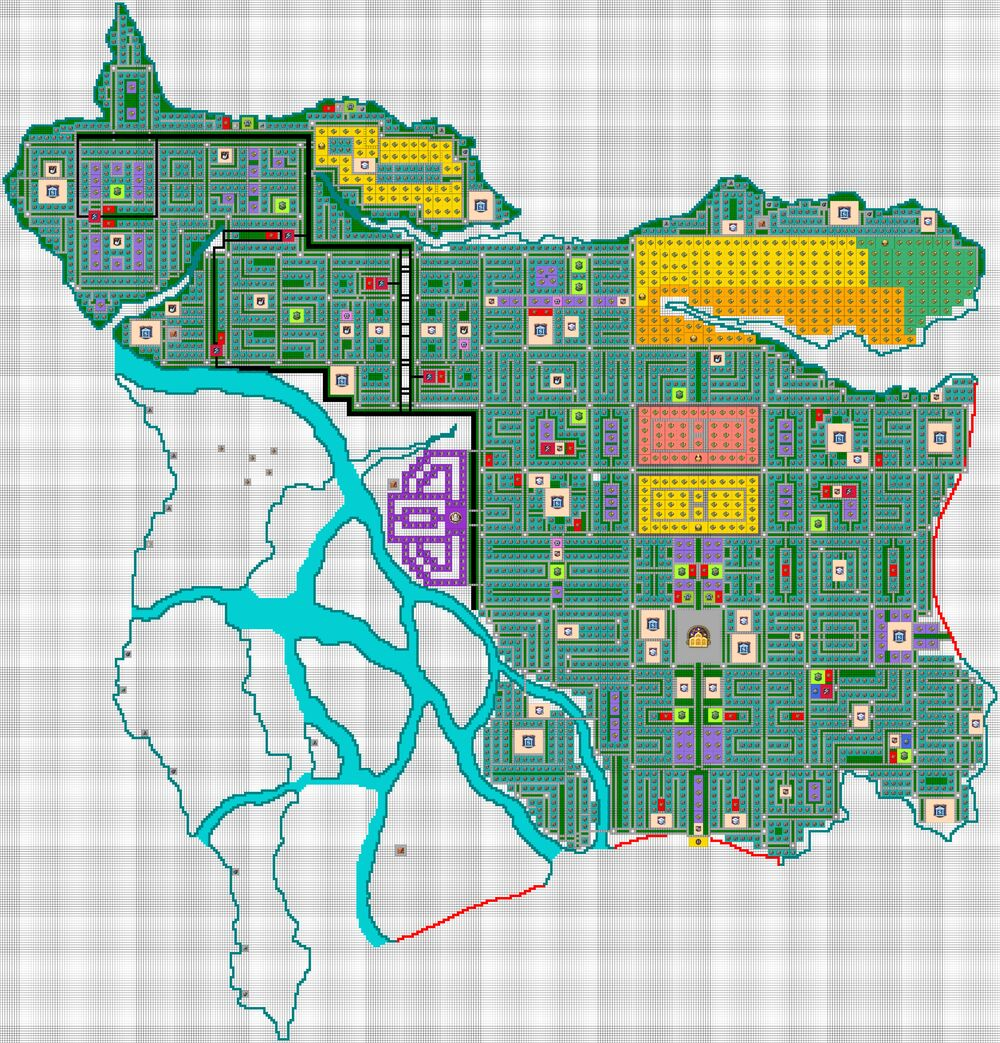
\includegraphics[scale=0.2]{analysis/figures/Leiden_8.jpg}
\caption{Write here the caption for the image.}
\label{fig:leiden}
\end{figure}


\noindent This research shows that for the Nothofagaceae treeline in New Zealand, the current treeline position is constrained by cold-induced photoinhibition effects linked to the surprising occurrence of frequent summer frosts at treeline. As F. cliffortioides is otherwise well-adapted for high altitude environments, suggesting that we will observe a rapid uphill encroachment once current limitations diminish in the face of global warming. Such empirical results, combined with greater use of agent-based modelling that incorporates fine-scale topographic maps and microhabitat heterogeneity will assist us to put individual tree performance in the context of large scale abiotic functional stress gradients and improve our understanding of alpine ecotone formation and maintenance.


Figures and tables can be referenced in LaTeX using the ref command, e.g. Figure \ref{fig:leiden} and Table \ref{tab:citytable}.\\
\\

%%%%% TABLE INSERT %%%%%%%%

\begin{table}[ht]
\caption{\label{tab:citytable} Legend title here.}
\centering
\begin{tabular}{|l|l|l|}  % l for left, c for center, r for right oriented
\hline
Country & City & Suburb \\
\hline
Germany & Bielefeld & Hillegossen \\
\hline
New Zealand & Auckland & Blockhouse Bay \\
\hline
\end{tabular}
\end{table}

\noindent This research shows that for the Nothofagaceae treeline in New Zealand, the current treeline position is constrained by cold-induced photoinhibition effects linked to the surprising occurrence of frequent summer frosts at treeline. As F. cliffortioides is otherwise well-adapted for high altitude environments, suggesting that we will observe a rapid uphill encroachment once current limitations diminish in the face of global warming. Such empirical results, combined with greater use of agent-based modelling that incorporates fine-scale topographic maps and microhabitat heterogeneity will assist us to put individual tree performance in the context of large scale abiotic functional stress gradients and improve our understanding of alpine ecotone formation and maintenance.







\section{Method}


\noindent This research shows that for the Nothofagaceae treeline in New Zealand, the current treeline position is constrained by cold-induced photoinhibition effects linked to the surprising occurrence of frequent summer frosts at treeline. As F. cliffortioides is otherwise well-adapted for high altitude environments, suggesting that we will observe a rapid uphill encroachment once current limitations diminish in the face of global warming. Such empirical results, combined with greater use of agent-based modelling that incorporates fine-scale topographic maps and microhabitat heterogeneity will assist us to put individual tree performance in the context of large scale abiotic functional stress gradients and improve our understanding of alpine ecotone formation and maintenance.



%%%% FIGURE INSERT %%%%%%%

\begin{figure}[ht]  %t for top, b bottom, h for right here after text
\centering % centers the picture
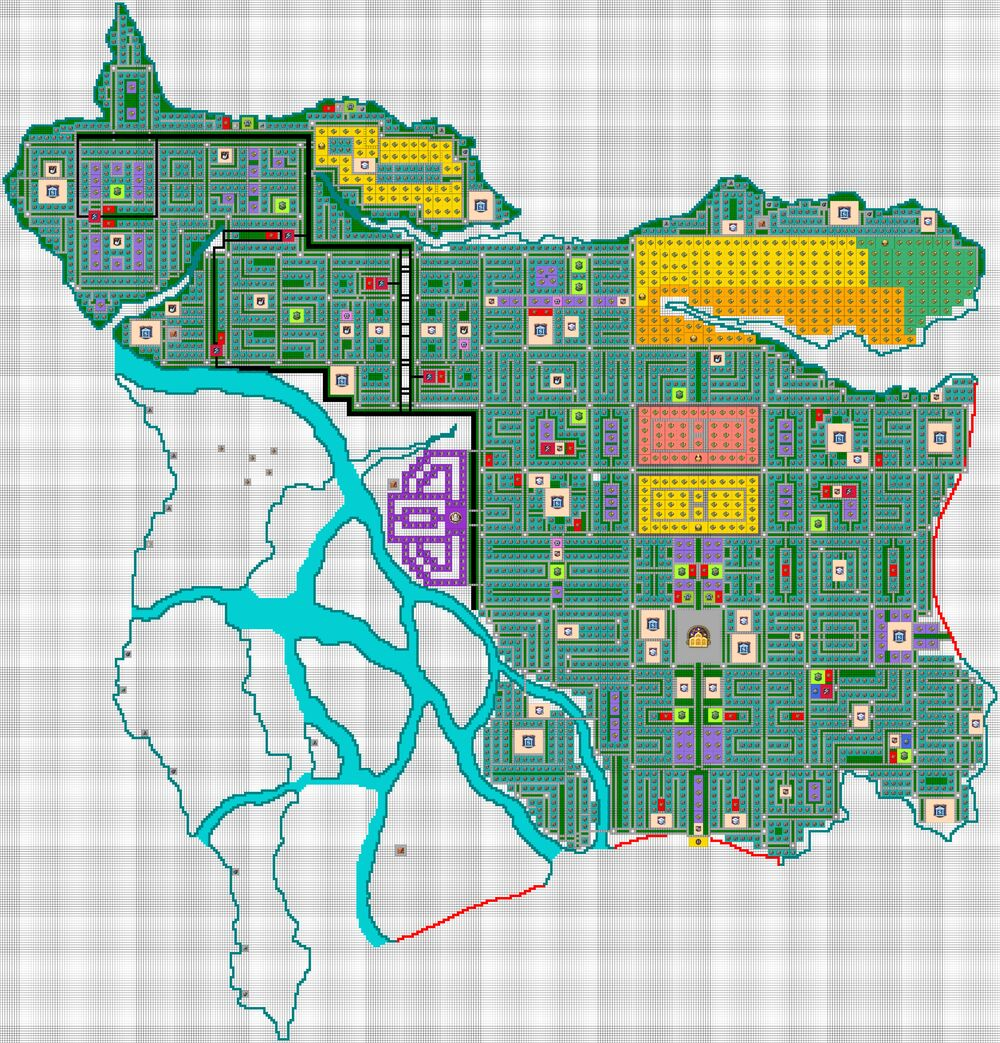
\includegraphics[scale=0.2]{analysis/figures/Leiden_8.jpg}
\caption{Write here the caption for the image.}
\label{fig:image}
\end{figure}


\section{Results}


\noindent This research shows that for the Nothofagaceae treeline in New Zealand, the current treeline position is constrained by cold-induced photoinhibition effects linked to the surprising occurrence of frequent summer frosts at treeline. As F. cliffortioides is otherwise well-adapted for high altitude environments, suggesting that we will observe a rapid uphill encroachment once current limitations diminish in the face of global warming. Such empirical results, combined with greater use of agent-based modelling that incorporates fine-scale topographic maps and microhabitat heterogeneity will assist us to put individual tree performance in the context of large scale abiotic functional stress gradients and improve our understanding of alpine ecotone formation and maintenance.



\section{Dicussion}


\noindent This research shows that for the Nothofagaceae treeline in New Zealand, the current treeline position is constrained by cold-induced photoinhibition effects linked to the surprising occurrence of frequent summer frosts at treeline. As F. cliffortioides is otherwise well-adapted for high altitude environments, suggesting that we will observe a rapid uphill encroachment once current limitations diminish in the face of global warming. Such empirical results, combined with greater use of agent-based modelling that incorporates fine-scale topographic maps and microhabitat heterogeneity will assist us to put individual tree performance in the context of large scale abiotic functional stress gradients and improve our understanding of alpine ecotone formation and maintenance.


\section{Wrap Text}


\begin{wrapfigure}{r}{0.7\textwidth}
  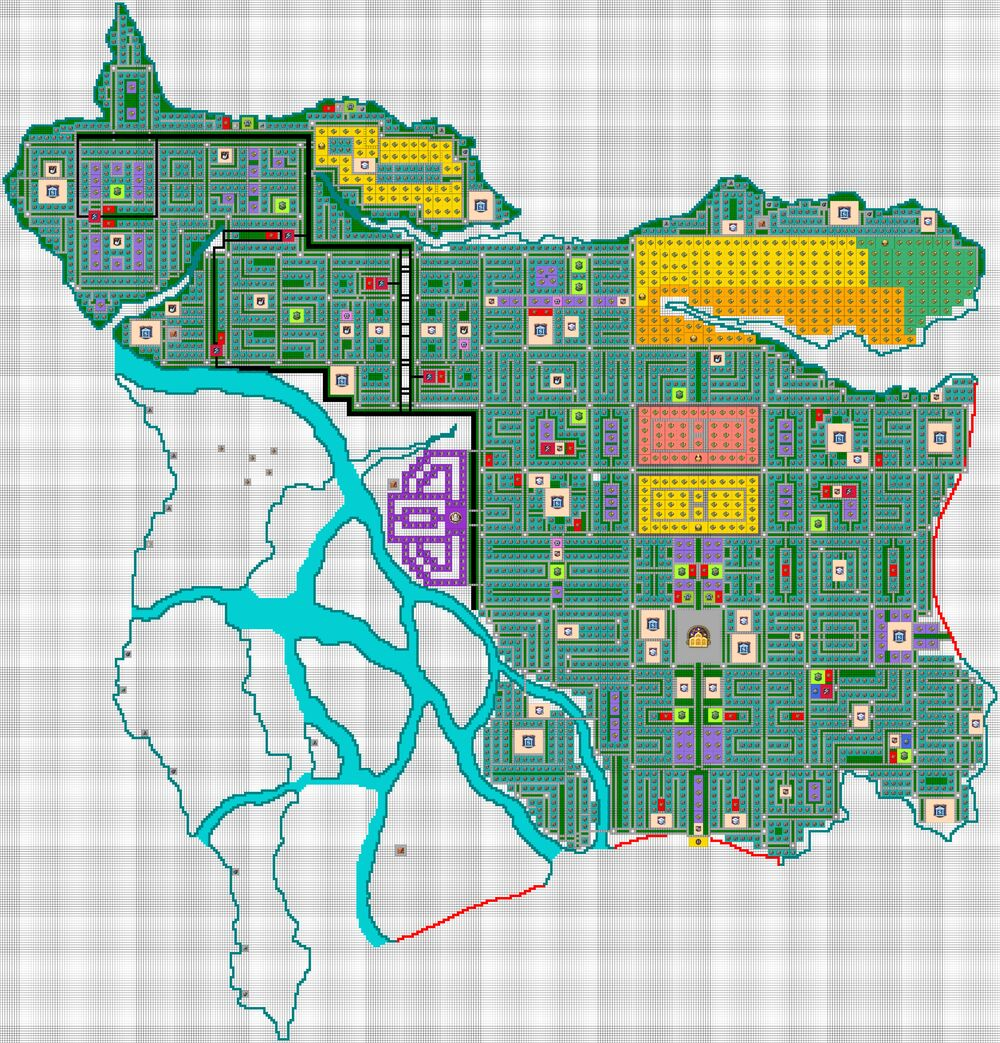
\includegraphics[scale=0.05, width=20mm]{analysis/figures/Leiden_8.jpg}
  \caption{Write here the caption for the image.}
  \label{fig:imagex}
\end{wrapfigure}




\noindent This research shows that for the Nothofagaceae treeline in New Zealand, the current treeline position is constrained by cold-induced photoinhibition effects linked to the surprising occurrence of frequent summer frosts at treeline. As \textit{F. cliffortioides} is otherwise well-adapted for high altitude environments, suggesting that we will observe a rapid uphill encroachment once current limitations diminish in the face of global warming. Such empirical results, combined with greater use of agent-based modelling that incorporates fine-scale topographic maps and microhabitat heterogeneity will assist us to put individual tree performance in the context of large scale abiotic functional stress gradients and improve our understanding of alpine ecotone formation and maintenance (For more info see \href{www.dragonfly.co.nz}{Dragonfly Website})



\printbibliography

\end{document}